%!TEX root = ./main.tex

\chapter{The quest for a faster kNN search} % (fold)
\label{sec:the_quest_for_a_faster_knn_search}

\section{A short evaluation of OpenCL and CUDA} % (fold)
\label{sub:a_short_evaluation_of_opencl_and_cuda}

% section a_short_evaluation_of_opencl_and_cuda (end)

\section{Investigation of a brute force approach based on Garcia} % (fold)
\label{sub:investigation_of_a_brute_force_approach_based_on_garcia}

% section investigation_of_a_brute_force_approach_based_on_garcia (end)

% Possible RQ for the k-d tree section.
\begin{myrq}
\label{rq:structure_aml}
    It is possible to use a k-d tree, to increase the performance of a large number of repeated, 3-d, low k queries in a large dataset.
\end{myrq}

 % Det finnes mange papers om alternativer til k-d tree som vi bør nevne i starten. eks. \cite{Owens:2007:ASO}  See page 7 av S12140-Superfast-Nearest-Neighbor-Searches-Using-Minimal-kd-Tree.pdf som ligger i git.

% A few different variations exist, but we will focus our explanation around a 2D example, storing point data in all nodes. The plane is split into two sub-planes along one of the axis (in our example the y-axis) and all the nodes are sorted as to whether they belong to the left or right of this split. To determine the left and right child of the root node, the two sub-planes are again split at an arbitrary point, this time cycling to the next axis (in our example the x-axis) and the

% In order to build a k-d tree for 3D space, you simply cycle through the three dimensions, instead of two.

% Given the previous splits and selection of nodes, the resulting binary tree would be as shown in the illustration under.

% Given that the resulting binary tree is balanced, we get an average search time for the closest neighbor in O(log2(n)) time. For values of k << n, the same average search time can be achieved, with minimal changes to the algorithm, when searching for the k closest neighbors. It is known from literature that balancing the tree can be achieved by always splitting on the meridian node. Building a k-d tree in this manner takes O(kn log2(n)) time.

% Interested readers is encouraged to look at the paper Multidimensional binary search trees used for associative searching by Jon Louis Bentley, where k-d trees first was described.

\section{Application of k-d trees to the kNN problem} % (fold)
\label{sub:application_of_kd_trees_to_the_knn_problem}

A usual strategy, when wanting to improve the performance of repeated queries in a large dataset, is to organize the dataset into some data structure especially suited for fast querying. When choosing this strategy, you are trading of the additional time penalty of building the data structure, for increased performance on each query, hopefully offsetting the build-time penalty. When considering the needs of TechnoSoft Inc, as described in section \ref{a_short_introduction_to_the_kNN_algorithm}, this strategy seems like a good fit.

In this section, we will present the k-d tree data structure, and show how it can be used for operating on three-dimensional point cloud data. Then an investigation is performed, in order to determine the possible benefits of a parallel k-d tree based algorithm.


\subsection{Building k-d trees for point cloud data} % (fold)
\label{ssub:building_k_d_trees_for_point_cloud_data}

A k-d tree can be thought of as a binary search tree in k dimensions. A binary search tree is constructed such that, for a given node, one of Its child-subtrees is consisting of elements smaller than the current node, and the other child-subtree is consisting of elements larger than the current node. The same strategy is applied when constructing a k-d tree, but at each level we are sorting the child-subtree elements according to one selected dimension, called the discriminant for this level. This discriminant is cycled through the different dimensions, as we move down each level in the tree. A formal description of k-d trees is given by Jon Louis Bentley in the paper Multidimensional Binary Search Trees Used for Associative Searching \cite{Bentley:1975:MBS:361002.361007}.

Let us have a look at an example using data for two dimensions. Figure \ref{fig:kd_tree_2d_plane} shows us a set of points on a two dimensional plane. The lines through each point indicate the split plane formed by the discriminant associated with the different points.

\begin{figure}[ht!]
\centering
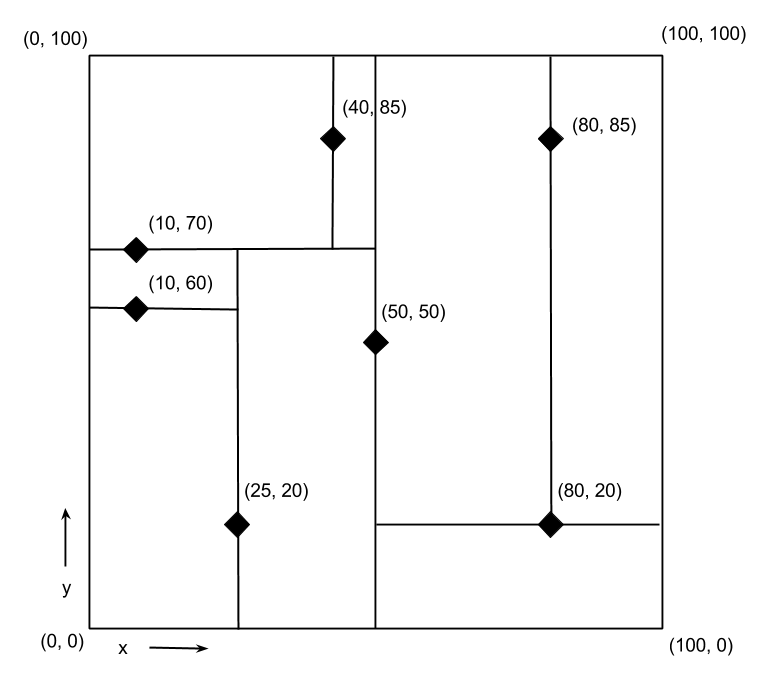
\includegraphics[width=120mm]{../gfx/kd_tree_illustration_graph.png}
\caption{A set of points on a plane, with a possible k-d tree indicated.}
\label{fig:kd_tree_2d_plane}
\end{figure}

The corresponding k-d tree is shown in figure \ref{fig:kd_tree_2d}. Note that lover values in each level are placed in the left branches, and higher values are placed in the right branches.

\begin{figure}[ht!]
\centering
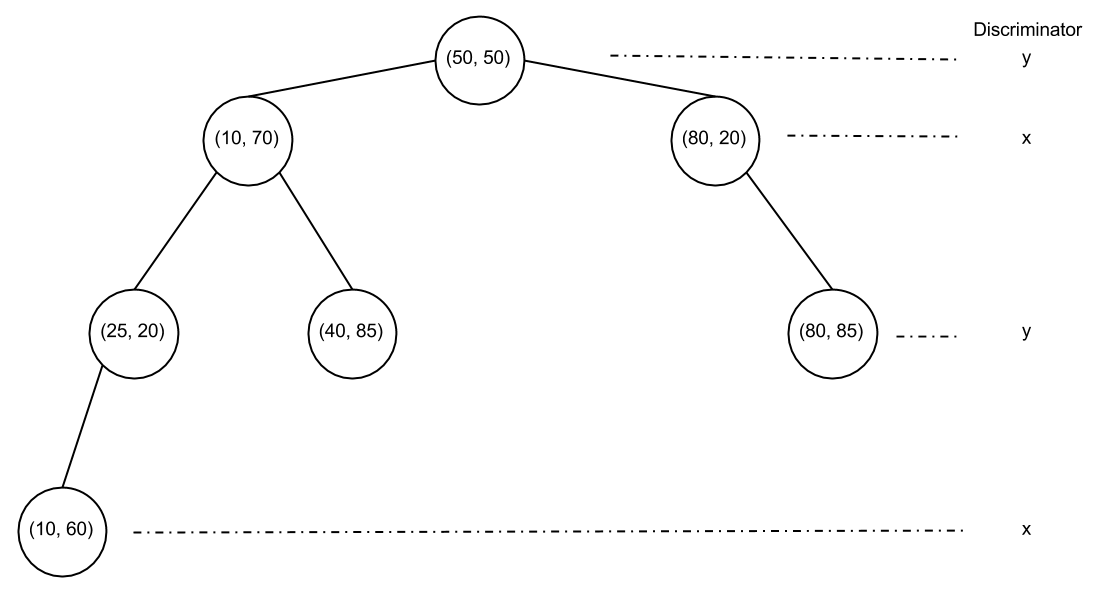
\includegraphics[width=120mm]{../gfx/kd_tree_illustration_tree.png}
\caption{Tree representation of the points in figure \ref{fig:kd_tree_2d_plane}.}
\label{fig:kd_tree_2d}
\end{figure}

By extending this example with three fixed dimensions for the spatial dimensions, x, y, and z, we get a k-d tree suitable for storing point cloud data.

It it possible to construct several algorithms for building k-d trees from a set of points, and one simple approach is using a recursive function. Algorithm \ref{alg:seriel_tree_build} shows pseudocode for such a simple tree building algorithm. In the pseudocode, we have chosen to represent the different dimensions as a natural number. This means that x is represented by 0, y is represented by 1, z is represented by 2 and so on. Given a set of point, $P$, in $k$ space, and a initial split dimension $i$, it constructs a balanced k-d tree.

\begin{algorithm}
\caption{Recursive k-d tree build}
\label{alg:seriel_tree_build}
\begin{algorithmic}
    \Function{Build-KD-Tree}{$P$, $i$}
        \If{$P.length = 0$} \Comment{We have reached the end of a branch}
            \State \textbf{return} NIL
        \Else
            \State $m \gets \text{Median}(P)$

            \State \text{Let $L$ be all elements of $P < m$ in dimension $i$}
            \State \text{Let $H$ be all elements of $P > m$ in dimension $i$}

            \State $i' \gets (i + 1) \bmod k$ \Comment{k = 3 for a three dimensional k-d tree}

            \State $m.left \gets \text{Build-KD-Tree}(L, i')$
            \State $m.right \gets \text{Build-KD-Tree}(H, i')$
        \EndIf
        \State \textbf{return} $m$
    \EndFunction
\end{algorithmic}
\end{algorithm}

Algorithm \ref{alg:seriel_tree_build} starts by checking if there is any more points left in $P$. If not, it returns NIL as an end of branch marker. If there still is points left, the algorithm selects the median point, $m$, as the root node. Then it sorts all remaining points into a collection of points lower than the median, $L$, and higher than the median, $H$. The dimension, $i$, is incremented, and the Build-KD-Tree function is called recursively on both collections of points. Finally the root node is returned, so it can be assigned as the child of its parent node, or be used as a global root node.

It is worth to note that the performance of this k-d tree build algorithm is sensitive to the choice of a median finding algorithm, since we will be querying for the median \BigO{n} times. Choosing to just sorting the collection $P$, and selecting the median from the middle of the sorted collection, will not give optimal results. Fortunately, several \BigO{n} median selecting algorithms exist \cite{Cormen:2001} (Get chapter citation), quickselect, being the choice for our initial implementations. This gives a algorithm with a time complexity of \BigO{k*n*log(n)} \cite{Friedman:1977}.

A final note about algorithm \ref{alg:seriel_tree_build}, is that it does not handles points with duplicate values in one dimension. If the algorithm where to be feed with a point collection where all points had the same value for x, it would not be able to handle it, since such a point does not explicitly belong in $L$ or $H$. Several modifications can be made to handle this case. We can choose to place all conflicting median points, exept one, in either $L$ or $H$. The problem with this solution, is that we are not guaranteed to get a balance tree. If we where to have a set of points, where all points where tha same, we would get a tree at all, but just one long branch of length n. Another strategy is to try to place the conflicting medians, equally in $L$ and $H$. This way the median we select will be the midmost element in the point collection, retaining the balance in the finished k-d tree. Given that we consider that duplicate median points can be located in both subtrees of a node, this will not affect search operations on the tree, as we will see later.
% subsection building_k_d_trees_for_point_cloud_data (end)


\subsection{Querying the k-d tree} % (fold)
\label{sub:querying_the_k_d_tree}

With a k-d tree we can perform efficient searches for the closest point to a given point in \BigO{n*log(n)} average time \cite{Friedman:1977}. By maintaining a collection of the k closest points during execution of the query, we can even perform kNN searches. An example of a kNN search algorithm is shown in listing \ref{alg:recursive_knn_kd_tree_search}.

(Something about how searching works in the general sense?)

The procedure will take the root of a k-d tree, $r$, a query point, for which we want to find the k closest points, an initial dimension, $i$, which should be the same as the one used to build the tree. It uses this data to manipulate a collection of the k closest points to $q$, stored in $K$.

In our example $K$ is a data structure with some special properties, called the k-heap. You can query it for the maximum distance value of the k points stored in it, and it will only store a predetermined number of points. If you try to insert more points than the predetermined number of points, it will discard the highest values, and only keep the k lowest values. This data structure can be easily implemented as a modified max-heap. When the size of the heap is lower than k, it it used in the usual manner, but when the heap is of size k, a slight modification to the insertion operation is made. Instead of adding the new element to the heap, the new element is swapped with the maximum value of the heap, if it is lower than this maximum value. Then the heap is re-balanced using standard algorithms. In our code, we assume the k-heap to be filled at the start with k points of either a random sample of points from the k-d tree, or with positive infinity. This way we do not need to take into account if the stack is filled yet, during the recursive execution of the procedure.

\begin{algorithm}
\caption{Recursive kNN k-d tree search}
\label{alg:recursive_knn_kd_tree_search}
\begin{algorithmic}
    \Procedure{kNN-KD-Tree}{$K, r, q, i$}
        \If{$r =$ NIL} \Comment{We have reached the end of a branch}
            \State \textbf{return}
        \EndIf

        \State $d \gets \text{Distance}(r, q)$
        \State $dx \gets r.x[i] - q.x[i]$

        \If{$d < K.max$} \Comment{Is $r$ closer to $q$ than the current k best points?}
            \State $r.distance \gets d$
            \State \text{Insert}($K, r$)
        \EndIf

        \State $i' \gets (i + 1) \bmod k$ \Comment{k = 3 for a three dimensional k-d tree}

        \If{$dx > 0$}  \Comment{Select $t$ and $o$ so we traverse towards closest point first}
            \State $t \gets r.left$, $o \gets r.right$
        \Else
            \State $t \gets r.right$, $o \gets r.left$
        \EndIf

        \State \text{kNN-KD-Tree}($K, t, q, i'$)

        \If{$dx^2 < K.max$} \Comment{Can there be closer points in the other subtree?}
            \State \text{kNN-KD-Tree}($K, o, q, i'$)
        \EndIf
    \EndProcedure
\end{algorithmic}
\end{algorithm}

Algorithm \ref{alg:recursive_knn_kd_tree_search} starts by checking if we have reached the end of a branch. If not, it calculates the Euclidean distance between the query point, $q$, and the current root point, $r$. Calculating this distance is a costly step, since it usually involves calculating a square root. This can be circumvented when implementing, by relying on using the square of the Euclidean distance as the distance metric, instead of the actual distance. This will not make a difference for the algorithm. The distance, $dx$, between the current root and the query point in dimension $i$ is also calculated.

The algorithm then checks if the current root point is closer to the query point than one of the points in the k-heap. If this is the case, it inserts the current root into the k-heap. The next dimension, $i'$, is calculated, and then the algorithm determines if it should traverse to the right or left child node first. For efficient querying, we want to traverse down the branch that would contain the query point. In other words, if the query point is lower than the current root point in the current dimension, we want to traverse to the left child, and vice versa. The child node that we want to traverse first, is often called the target, and its corresponding subtree is often called the target subtree. In the algorithm the symbol $t$ is used to represent target. The child and child-subtree that is not chosen for immediate traversal is called other and other-subtree. In the algorithm the symbol $o$ is used to represent other. The ability to prune away the other subtree, given our current best estimates stored in the k-heap and the distance $dx$, is what makes the k-d tree efficient for kNN searches.

After recursively investigating the target subtree, we ask if our estimates in the k-heap is better than the distance $dx$, remembering that the distances stored in the k-heap is squared. If this is the case, we know that there cannot be a closer point in the other subtree, and we can prune it from our search. If not, we have to check the other subtree as well. When the procedure terminated, the k closest points to the query point is stored in the k-heap.
% subsection querying_the_k_d_tree (end)

\subsection{Testing a serial k-d tree based kNN solver} % (fold)
\label{sub:testing_a_serial_k_d_tree_based_knn_solver}

In order to gain some idea about the possible performance of using
 
\begin{figure}[ht!]
\centering
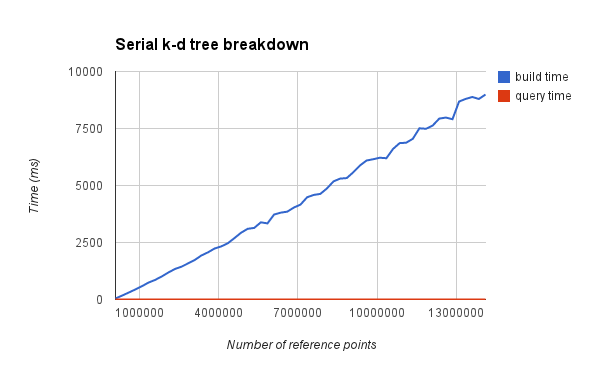
\includegraphics[width=120mm]{../gfx/serial-k-d-tree-breakdown.png}

\caption{serial-k-d-tree-breakdown}
\label{fig:serial_kd_tree_breakdown}
\end{figure}

Results:

As expected, almost all the time is spent building the tree. Querying for the closest neighbor in the largest tree took less than 0.0015 ms, but 9 seconds is a long time to wait for the tree to build.

The paper Real-Time KD-Tree Construction on Graphics Hardware - Kun Zhou et al. offers interesting, although slightly complex, ideas to an efficient parallelization of k-d tree construction. I order to save time, a good amount of time was spent searching for, and trying out, different open source implementations based on this paper. This search was unsuccessful. All the implementations we managed to find was problematic due to lack of updates, often not updated since 2011, and still running on CUDA 4.1, lack of documentation, lack of generalization or dubious source code.

A more uplifting find was several references to Real-Time KD-Tree Construction on Graphics Hardware in material published by Nvidia, regarding their proprietary systems for ray tracing. A graphics rendering technique often reliant on k-d trees, and indeed dependent on high performance.

Finding a way to represent the kd-tree boils down to representing a binary tree. This can be done in several ways, but we had some criteria for our representation:

\begin{itemize}
    \item The kd-tree should be memory-efficient, at best explicitly storing only the actual point coordinates. This since we want to store the largest possible amount of points on the smaller memory of the GPU.
    \item The kd-tree representation should be easy to split, distribute and join, since we want to build it on several independent processes.
\end{itemize}

After a bit of research and trial and error, we choose to represent the kd-tree as a array of structs, representing points, with an x, y and z coordinate stored in an short array. In order to turn this array into a binary tree, the following scheme was derived. Given an array, the root node of that array is the midmost element (the leftmost of the two, given an even number of elements). To find the left child of the root, you simply find the midmost element of the left sub-array, and likewise for the right child. This representation have some advantages and drawbacks.

Advantages:
\begin{itemize}
    \item Can represent binary trees where not all leaf-nodes are present. This is the minimal requirement for representing perfectly balanced k-d trees.
    \item Joining or splitting subtrees is as simple as appending or splitting arrays.
    \item Minimal memory overhead, k-d trees can even be built in-place on the array.
\end{itemize}

Drawbacks:
\begin{itemize}
    \item Cannot represent imperfectly balanced k-d trees. This mens that the median cannot be calculated through heuristic methods, but enforces a tree optimized for fast queries.
    \item Location of children and parents have to be recalculated for all basic traversing of the tree, with may reduce the performance of queries on the tree. In order to eliminate this drawback, a index cache is computed before the search is performed.
\end{itemize}

Given this representation of the kd-tree, the base kd-tree building algorithm can be expanded to the following:

Steps:
\begin{enumerate}
    \item Find the exact median (of the current split dimension) in this sub-array, and swap it to the midmost place.
    \item Go through all elements in the list, and swap elements, such that all elements lower than the median is placed to the left, and all elements higher than the median is placed to the right.
    \item Repeat for the new sub-arrays, until the entire tree is built.
\end{enumerate}

Results:

The serial kd-tree build times was similar or better than the base algorithm, so it is not discussed here

\begin{figure}[ht!]
\centering
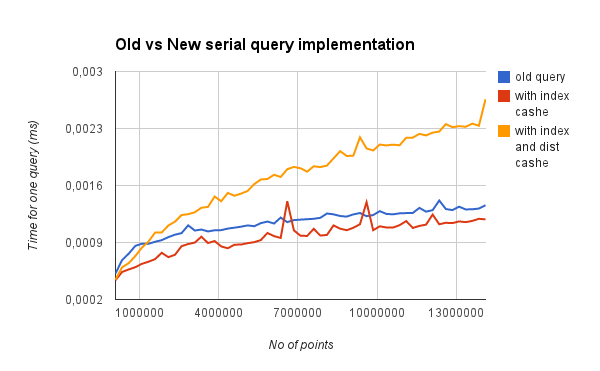
\includegraphics[width=120mm]{../gfx/awg-query-time-old-vs-new.png}

\caption{Awg query time old vs new}
\label{fig:awg_query_time_old_vs_new}
\end{figure}

The graph shows that our serial implementation of search in this data structure, given a pre-calculated index cache, is as fast, or slightly faster than the base algorithm. The possibility of improving the search even more, by storing all calculated distances in a distance cache was also explored, but we can see from the graph that the overhead associated with this operation did outweigh the benefits.

Some instability is apparent in the graph, but this is probably due to the author running other programs in the background when performing the test.

\begin{figure}[ht!]
\centering
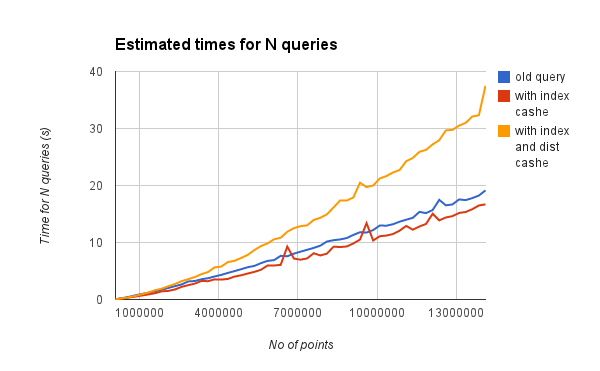
\includegraphics[width=120mm]{../gfx/n-query-time-old-vs-new.png}

\caption{n query time old vs new}
\label{fig:n_query_time_old_vs_new}
\end{figure}

The trend is exaggerated when considering N searches. Searching with an index cache is overall fastest, and gives a total search time of ~17 s for 14 million searches in a point cloud of 14 million.


% subsection testing_a_serial_k_d_tree_based_knn_solver (end)




% \subsection{The serial base algorithm} % (fold)
% \label{ssub:the_serial_base_algorithm}

% \begin{enumerate}
%     \item Build a balanced k-d tree from the point cloud.
%     \item Query the tree for different sets of neighbors.
% \end{enumerate}

% Time complexity:

% Steps:
% \begin{enumerate}
%     \item O(n log2 n). Achieving this speed is dependent on an efficient algorithm for finding the meridian.
%     \item Approximately O(log2 n), but dependent on size of k.
% \end{enumerate}


% \section{Development of a parallel kd-tree build algorithm} % (fold)
% \label{sub:development_of_a_parallel_kd_tree_build_algorithm}
% 
As noted in the previous section, the k-d tree build process is by far the most expensive operation, and we would save a lot of time by managing to parallelize it. One could think, why not use the serial build algorithm. This is a intuitive choice, but in a CUDA context a recursive algorithm is hard to parallelize. CUDA is based on a massive number of lightweight threads, and to get a fast algorithm one have to split the work between as many threads as possible. This is only possible if it is easy to split and divide the work to independent subtasks. In a recursive context this is hard, because a algorithms execution flow in hidden inside a threads call stack. This makes it hard for other threads to get the information needed to participate. The opposite of a recessive algorithm in an iterative approach, with have a more globally accessible execution flow. This introduces a new resource question.

\begin{myrq}
\label{rq:parallel_build}
    It is possible to parallelize the k-d tree build algorithm, in such a way that it gives a significant speed improvement compared to the serial algorithm.
\end{myrq}

In order to investigate RQ \ref{rq:parallel_build}, we have to look a bit closer at the different steps of the k-d tree build algorithm and look at different parallelization strategies.

Steps:
\begin{enumerate}
    \item Find the median of the points along a specified axis. This median point becomes the value of the current node.
    \item Sort all points with lower values than the median to the left of the median, and all the points with higher values than the median to the right.
    \item Perform this algorithm recursively on the left and right set of nodes.
\end{enumerate}

If we analyze the algorithm \ref{alg:seriel_tree_build}, we can see that for each node in the k-d tree a median finding and a partition has to be made, as described in step 1 and 2. We can call this recursive step a node task. The node task has to be done for all nodes starting at the root and successively go down the tree.



\subsubsection{Parallelization strategy} % (fold)
\label{ssub:parallelization_strategy}


First a good overall parallelization strategy has to be found. A good strategy manage to easily split the main task into small individual subtasks. From the serial recursive algorithm \ref{alg:seriel_tree_build}, we see that there are two recursive calls. This is logical, because we are building a binary tree.  The interesting observation is that a node task is only dependent on the parent node tasks. This means that each tree level are independent, which acts as a good start for our parallelization strategy.

Some other small observation, in regard of a parallelization strategy, is that all subtrees in the k-d tree generation are independent. Hence, the tree corresponding to the left and right child of a node can be done in parallel without any communication. The data is also independent, as a result of how we represent the tree as an array. By data independent, it is meant that the data structure easily can be partitioned to each subtask. In our case will the tree array successively be partitioned into contentious sublists, one for each node task.

From these observations, several strategies can be used to parallelize the k-d tree build algorithm. From the first observation a trivial strategy is to divide the tree levels into dependent tasks, where each node task in a tree level is a independent subtask. This gives us an power of two increasing number of parallel nodes tasks as we increase the tree level. The sublist size will decrease with a factor of two in each downward step. An other strategy is to parallelize each node task.

Both strategies can be used in conjunction with each other. The parallel node task algorithm can be used to speed up the early iterations, where the amount of node task in a tree level is small. As well as further parallelize the subtasks in later tree level iterations. This strategy also fit well to our choice of tree representation. One parallel operation can now take the tree array, split the tree into the current subtrees, perform the node task in each subtree in parallel, and the next tree level is created. All can be done inplace, so the algorithm is as memory efficient as possible.


% subsubsection parallelization_strategy (end)

\subsubsection{From recursive to iterative implementation} % (fold)
\label{ssub:from_recursive_to_iterative_implementation}

\begin{algorithm}
\caption{Iterative k-d tree build}
\label{alg:iterativ_tree_build}
\begin{algorithmic}
    \Function{Build-KD-Tree}{$Tree$}
        \ForAll {$level \in \text{all levels in } Tree$}
            \ForAll{$node \in level$}
                \State $dimension \gets |level| \bmod k$ \Comment{k = 3 for a three dimensional k-d tree}
                \State $\text{Balance-node}(node, dimension)$
            \EndFor
        \EndFor
    \EndFunction
\end{algorithmic}
\end{algorithm}


% subsubsection from_recursive_to_iterative_implementation (end)




% TODO: Header must be improved
\subsubsection{Selecting an algorithm} % (fold)
\label{ssub:selecting_a_algorithm}



As we have seen in section \ref{sub:application_of_kd_trees_to_the_knn_problem}, many algorithms for finding median exist. Since we now want to implement the algorithm with CUDA, the environment has changed, and quick select may not be the best alternative anymore. The first problem with quick select is that it is recursive, which makes it hard to parallelize on CUDA. Therefor it may be profitable to look at other, more parallelization, algorithms.


First a reuse of the bitonic sort was investigated. Given a sorted list one can find the median directly, by simply looking at the midmost element of the array. The partitioning is also done in the process. Unfortunately this strategy proved unsuccessful, as re-purposing the bitonic algorithm for such an task proved difficult. The reason for this is that a pure bitonic sort only manage to sort lists with a length of power of two. The normal solution is to create a longer list then needed, which destroys many of the advantages with our binary tree representation. There are also other solutions to the problem, for example one by K.E. Batcher \cite{Batcher:1968}, but these solutions introduces a lot of divergence that destroys performance on the GPU. We also have the inherent downside of sorting a list in order to find the median, since \BigO{n} algorithms for finding the median exist, compared to the \BigO{n log(n)} time required by sorting.


The existing linear algorithms for finding the median is mostly based on a more generic problem, namely selection or k'th order statistic algorithms \citep[Chapter 9]{Cormen:2001}. Our serial choice, Quick select, is one of these. It is possible to implement a iterative version, so that the bad properties from the recursive version are eliminated. This option was ignored, because literature states that there are other better suited algorithms, like Alabi \citep{Alabi:2012}. Alabi goes through the radix select and bucket select algorithm in detail. The big difference between them is the constant time penalty. The radix sort have a more exact time complexity of \BigO{bn}, where b is the number of bits in each number. While the penalty for bucket select is \BigO{an}, where $a$ stands for the degree of agglomeration in the values. The algorithm is week when the points are clusters together. His results shows that bucket select normally is slightly faster, except when $a$ is high. Although bucket select normally have better results, we expect a high degree of agglomeration in our application, so we choose radix select.


\subsubsection{Radix select} % (fold)
\label{ssub:radix_select}

% subsubsection radix_select (end)

The radix select is based on a bitwise partitioning, much like radix sort \cite[Chapter 8.3]{Cormen:2001}. In each step, elements are partitioned in two subgroups based on the current bit. Then the subgroup that contains the median is determined, and the search continue in that subgroup until the median is found.

\begin{figure}[ht!]
\centering
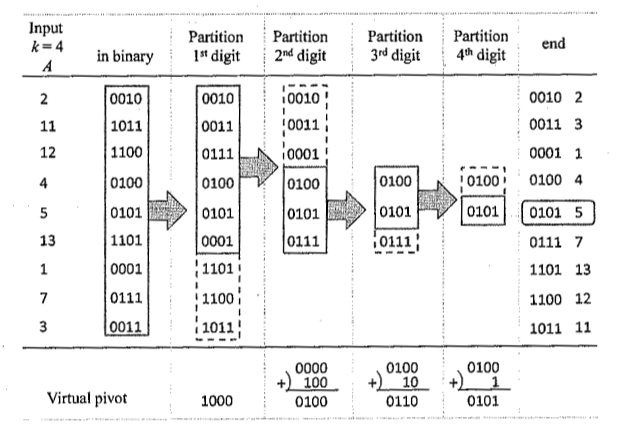
\includegraphics[width=100mm]{../gfx/Radix_select.png}

\caption{An illustration of radix selection \cite{cayman:2012}.}
\label{fig:radix_select}
\end{figure}

When it comes to create a parallelization strategy for radix select it is first advisable to take a look at a highly optimized radix sort like, \citep{MerrillG11}. The radix select can easily be reduced from a radix sort, and many concepts can therefore be reused. An other interesting implementation is the radix select from \citep{Alabi:2012}. They both uses a intuitive parallelization strategy by splitting each radix partition into parallel operations. The way our and Alba's solution differs from Merrill is firstly that we start on the most significant digit, since a least significant digit approach will not reduce the problem in each step. Secondly we only iterate on the digit which contains the median, and let us reduce the problem in each iteration.

Our radix select is a slightly modified version in three ways. We want to solve the node task, which forces us to also partition the list around the median. The algorithm also need to work in a inplace fashion. The last modification, is that our parallel operation must to several radix selections at once, at different parts of the main tree array.


\subsubsection{Our implementation} % (fold)
\label{ssub:our_implementation}


- split up the work in respect to cuda
- Pseudocode
- forklarting av cuda
- diskutere minnebruk. shared memory
- divergence
-



% subsubsection our_implementation (end)





% It is hard to use all the parallel power of cuda in this algorithm. The reason is that the problem is divided in three different types; partition one huge list, partition some middle sized list and partition many small lists. This is the reason why we have chosen to use three different implementation of k'th order statistic. The constant time penalties of the two algorithms we have chosen give us a clear indication the radix select is best on large lists while quick select is best on small lists.

% Results:
% \begin{figure}[ht!]
% \centering
% 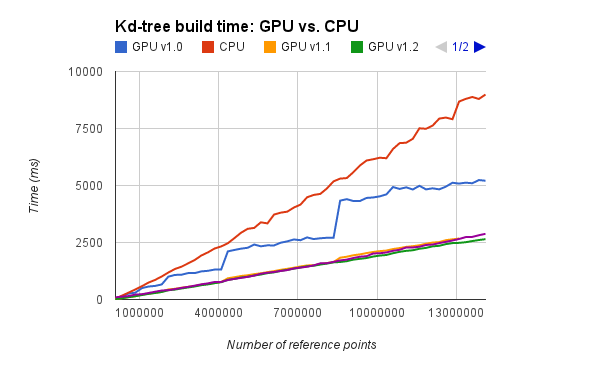
\includegraphics[width=120mm]{../gfx/gpu-vs-cpu-build-time.png}

% \caption{GPU vs CPU build time.}
% \label{fig:sublime_ide}
% \end{figure}

% We see that the parallel implementation performs better than the base serial implementation, building a tree of 14 million points in just over 5 seconds, compared to just under 10 required by the serial algorithm. Still we regard this as a quite rough implementation, in need of more tuning to really bring out the speed potential. The potential for parallelizing the workload for the first and last iterations have not been fully developed. This is due to the implementation forcing one version of the radix select algorithm being to work on all problem sizes. This is not optimal for dividing cuda resources, and as a result, we get high penalties when the problem size reaches unsuitable values.

% We also see a couple of large jumps in the graph. This happens when the number of elements passes a power of two and the height of the resulting k-d tree increase. The height increase hits the implementation at its weakest.

% Tuning the algorithm to alternate between radix select and quick select, eliminates this problem, as is visible in the graph for GPU v1.1. This removes the penalty for calculating the median at unsuitable problem sizes, giving an build time of ~2.4 seconds for 14 million points, compared to the ~9 seconds required by the serial implementation, or the ~5.2 seconds required by the old parallel implementation.

% % subsubsection selecting_a_algorithm (end)
% Memory usage:

% To analyses the space complexity of the k-d tree build and search algorithm, we have made an theoretical calculation of both algorithms GPU memory consumption, and tested it against results from a GeForce 560ti and a Nvidia grid K520 (amazon web service delved).

% It is important to note that the only hard memory limitation is related to building the tree, as a search for N query-points can be performed in several operations. If you e.g. run into memory limitations when searching for pow(10, 8) query-points, you can simply perform two searches on pow(5, 8) query-points to get around the limitation. Loading the pre-built k-d tree on the GPU for searching, and performing one query for a low value of k, will always consume less memory than building the actual k-d tree.

% **Kd-tree-build**

% The memory consumption for the k-d tree build is only depended on the number of points (n) and the theoretical consumption rate grows linearly as \BigO{36n} subset of \BigO{n}.

% \begin{figure}[ht!]
% \centering
% 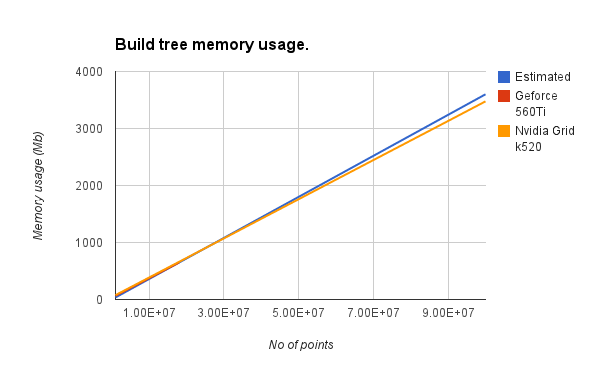
\includegraphics[width=120mm]{../gfx/memory-usage-build.png}

% \caption{Memory usage of k-d tree-build.}
% \label{fig:memory_usage_build}
% \end{figure}

% We see that the estimation fit the real consumption almost perfectly, and with this memory model, we can easily estimate the GPU memory requirements for different problem sizes.

% Given that a customer wants to perform a knn-search on a point cloud of 100 million, he or she would need a GPU with at least 3.6 Gb of spare memory. Under we have tabulated what maximum problem sizes you would expect to be able to run on a selection of Nvidia graphics cards:

% \begin{center}
%     \begin{tabular}{ | l | l | p{5cm} |}
%     \hline
%     Nvidia GPU & Available memory & Maximum problem size \\ \hline
%     GTX TITAN & 6144 MB & 1.79E+08 \\ \hline
%     GTX 780 & 3072 MB & 8.95E+07 \\ \hline
%     GTX 770 & 2048 MB & 5.97E+07 \\ \hline
%     Quadro K6000 & 12288 MB & 3.58E+08 \\ \hline
%     Quadro K5000 & 4096 MB & 1.19E+08 \\ \hline
%     Quadro K4000 & 3072 MB & 8.95E+07 \\ \hline
%     Tesla K40 & 12288 MB & 3.58E+08 \\ \hline
%     Tesla K20 & 5120 MB & 1.49E+08 \\ \hline
%     \end{tabular}
% \end{center}

% These numbers should be read as rough estimates, as each card is expected to have internal processes requiring an unspecified constant amount of the available memory, therefor lovering the maximum problem size possible to run on these cards in practice. It is also worth to mention that when buying a GPU for GPGPU tasks, other performance characteristics is equally, or more, important.

% **Kd-search**

% The kd-search is used to query every point against each other. It has a theoretical memory consumption rate at \BigO({40+4k}n) subset of \BigO{kn}. The consumption is therefore depended on the number of points (n) and the number of neighbors (k).

% \begin{figure}[ht!]
% \centering
% 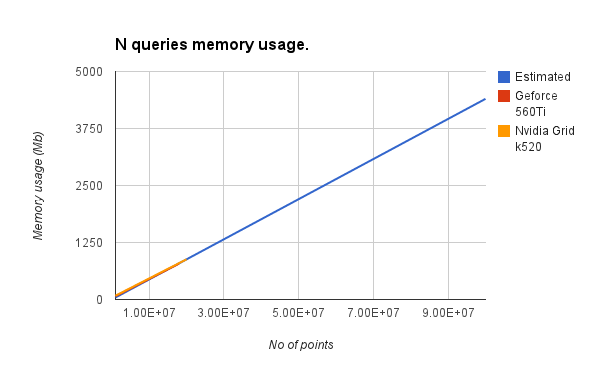
\includegraphics[width=120mm]{../gfx/memory-usage-kd-search.png}

% \caption{Memory usage of kd-search.}
% \label{fig:memory-usage-kd-search}
% \end{figure}

% Also in this case our estimation fit the real consumption with a high degree of accuracy.

% Further work:
% \begin{itemize}
%     \item Look at memory optimization.
%     \item Improve utiliti methods like: accumulateindex, minReduce.
%     \item Forloop Unrolling.
% \end{itemize}

% % section development_of_a_parallel_kd_tree_build_algorithm (end)

% \section{Development of a parallel kd-tree search algorithm} % (fold)
% \label{sub:development_of_a_parallel_kd_tree_search_algorithm}

% \section{The quest for a fast KNN search} % (fold)
% \label{sec:the_quest_for_a_fast_KNN_search}

% Our initial investigation led us to believe that a serial implementation could be as fast as the parallel brute-force solution, for point clouds with fewer than 1 000 000 points, given that both algorithms start with an unordered set of points. Reimplementing the brute-force algorithm with bitonic sort, and optimizing for three dimensions, has shown us that this initial belief was unsupported, and currently the brute force algorithm is faster when starting from a unorganized set of points. When considering repeated querying of the same point cloud, the k-d tree based solution pulls ahead, as most of its running time is spent building the k-d tree for querying. If building the k-d tree could be parallelized this could change. although documented in literature, such an parallelization is still elusive.

% In order to make the document more readable, we have included short descriptions of the algorithms used, a short reference to theoretical time complexity. We then go on to list our current results, problematic areas and possible improvements.

% The following papers, available in the resources folder, forms the literary basis for our current work.

% Related to the brute force approach:
% \begin{itemize}
%     \item Improving the k-Nearest Neighbor Algorithm with CUDA - Graham Nolan
%     \item Fast k Nearest Neighbor Search using GPU - Garcia et al.
%     \item K-nearest neighbor search: fast gpu-based implementations and application to high-dimensional feature matching - Garcia et al.
% \end{itemize}

% Related to the k-d tree based approach:
% \begin{itemize}
%     \item Real-Time KD-Tree Construction on Graphics Hardware - Kun Zhou et al.
% \end{itemize}


% \section{Brute force based effort} % (fold)
% \label{sub:brute_force_based_effort}

% \subsection{Garcia's base algorithm} % (fold)
% \label{ssub:garcias_base_algorithme}

% Garcia's algorithm is based on a naive brute-force approach. It consists if two steps:
% \begin{enumerate}
%     \item Calculate the distance between all reference points and query points.
%     \item Sort the distances and pick the k smallest distances.
% \end{enumerate}

% Garcias implementation supports any number of dimensions, reference points and query points (or up to ~65000, number of blocks in the GPU). Due to this feature the algorithm use a lot of extra computation power when only one query point and a small dimensions is selected.

% Time complexity:

% Steps:

% \begin{enumerate}
%     \item O(n). Every reference point must be evaluated once. Since all calculations are independent, we have a large potential for parallelizing.
%     \item Insertion sort: O(pow(n, 2)).
% \end{enumerate}
% % subsection garcias_base_algorithme (end)

% \subsection{Our reimplementation} % (fold)
% \label{ssub:our_reimplementation_2}

% Bitonic-sort:

% Graham Nolan discusses the possibility of improving Garcia's algorithm by reimplementing step two with a bitonic sort. His source code has not been available to us, but he states that the run-time improvements was significant. As well as choosing bitonic sort for the sorting stage of our algorithm, our implementation supports up to 15 000 000 points before memory errors occur, and we have limited the number of dimensions to three.

% Time complexity:

% Steps:
% \begin{enumerate}
%     \item O(n).
%     \item Bitonic sort: worst case = O(n * log2(n)), average time ( parallel) = O(log2(n)).
% \end{enumerate}

% Results:

% Testing the different algorithms for a range of point cloud sizes and a fixed value for k, gave the following results.

% \begin{figure}[ht!]
% \centering
% 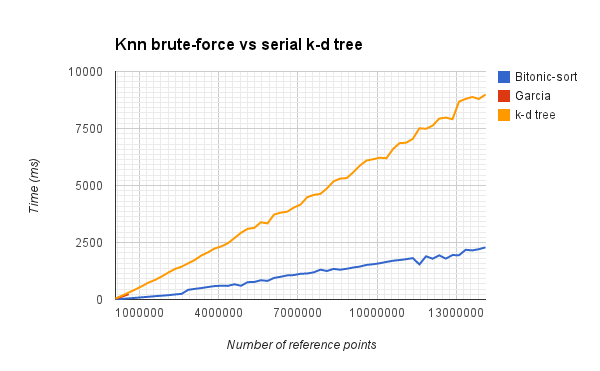
\includegraphics[width=120mm]{../gfx/knn-brute-force-vs-serial-k-d-tree.png}

% \caption{knn-brute-force-vs-serial-k-d-tree.png}
% \label{fig:knn_brute_force_vs_serial_k_d_tree}
% \end{figure}

% We see that our reimplementation of the brute-force algorithm performs well overall, notably improving on Garcia's implementation (only visible as a short line in the beginning of the graph, due to the restricted number of points it is able to compute). Still more speed is desired before good interactive usage can be achieved.

% Test with n = 8 388 608:

% \begin{itemize}
%     \item Memory transfer 21.1 ms
%     \item Calculate all distances 2.5 ms
%     \item Bitonic sort 176 ms
%     \item Total 200 ms
% \end{itemize}

% Min-Reduce:

% An other possibility to improve step 2 is to use a reduce operation to get the smallest distances. This can be done k times to get the k smallest values.

% Time complexity:

% Steps:

% \begin{enumerate}
%     \item O(n).
%     \item Min-reduce: k* log2(n)).
% \end{enumerate}

% Memory optimalisation:

% We have done some memory optimization based on a
% %[presentation](https://github.com/hgranlund/tsi-gpgpu/blob/master/resources/kNN/reduction.pdf)
% from Nvidia.

% The optimizations include:

% \begin{itemize}
%     \item Shared memory utilization.
%     \item Sequential Addressing.
%     \item Complete for-loop Unrolling.
% \end{itemize}

% \begin{figure}[ht!]
% \centering
% 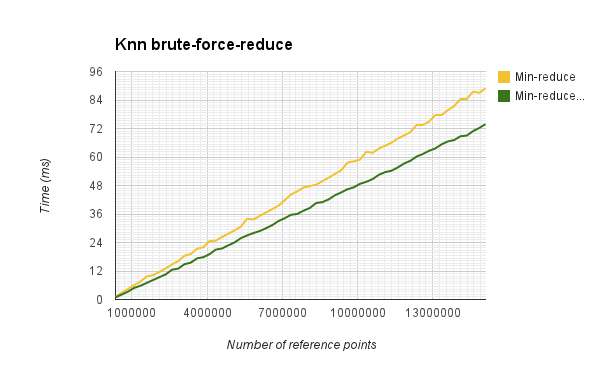
\includegraphics[width=120mm]{../gfx/knn-brute-force-reduce-memory-opt.png}

% \caption{Comparison between knn-brute-force-reduce with and without memory optimizations (k=10).}
% \label{fig:knn_brute_force_reduce_memory_opt}
% \end{figure}

% Results:

% Test results of n = 8 388 608 with no memory optimization:
% \begin{itemize}
%     \item Memory transfer:  21.1 ms.
%     \item Calculate all distances: 2.5 ms
%     \item One min-reduce step : 4.8 ms.
%     \item Total time: (23.7 + k*4.8) ms.
% \end{itemize}

% Test results of n = 8 388 608 with memory optimization:
% \begin{itemize}
%     \item Memory transfer:  21.1 ms.
%     \item Calculate all distances: 2.5 ms
%     \item One min-reduce step : 1.7 ms.
%     \item Total time: (23.7 + k*1.7) ms.
% \end{itemize}

% \begin{figure}[ht!]
% \centering
% 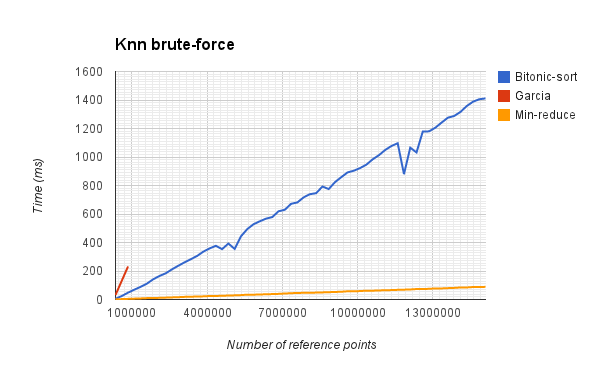
\includegraphics[width=120mm]{../gfx/BitonicVSreduce.png}

% \caption{Comparison between bitonic and reduce (k=10).}
% \label{fig:bitonic_vs_reduce}
% \end{figure}

% Possible improvements:

% \begin{itemize}
%     \item Memory improvements. Use shared memory and texture memory.
%     \item Modify bitonic sort, so do not need to sort all points. We can split the distance array to fit into the GPU blocks, move the smallest values in each block, then sort the moved values. ~O((n/b)* b*log2(b)) subsetof O(n/b), b = Number of threads in each block, n= number of reference points
%     \item Replace bitonic sort with min reduce. O(k*log2(n)).
% \end{itemize}
% subsection our_reimplementation (end)
% section brute_force_based_effort (end)

% \section{KD-tree based effort} % (fold)
% \label{sub:kd_tree_based_effort}

% A k-d tree can be thought of as a binary search tree for graphical data. A few different variations exist, but we will focus our explanation around a 2D example, storing point data in all nodes. The plane is split into two sub-planes along one of the axis (in our example the y-axis) and all the nodes are sorted as to whether they belong to the left or right of this split. To determine the left and right child of the root node, the two sub-planes are again split at an arbitrary point, this time cycling to the next axis (in our example the x-axis) and the

% \begin{figure}[ht!]
% \centering
% 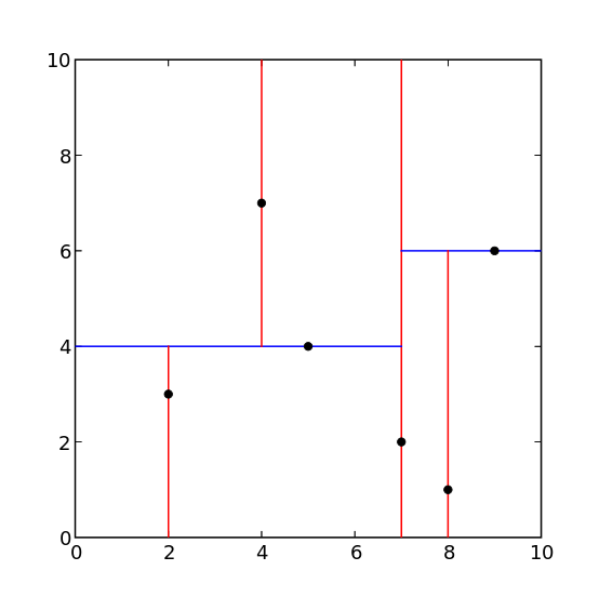
\includegraphics[width=120mm]{../gfx/Kdtree_2d.png}

% \caption{2D KD-tree}
% \label{fig:kdtree_2d}
% \end{figure}

% In order to build a k-d tree for 3D space, you simply cycle through the three dimensions, instead of two.

% Given the previous splits and selection of nodes, the resulting binary tree would be as shown in the illustration under. (All illustrations gratuitously borrowed from
% %[Wikipedia](http://en.wikipedia.org/wiki/k-d_tree))

% \begin{figure}[ht!]
% \centering
% 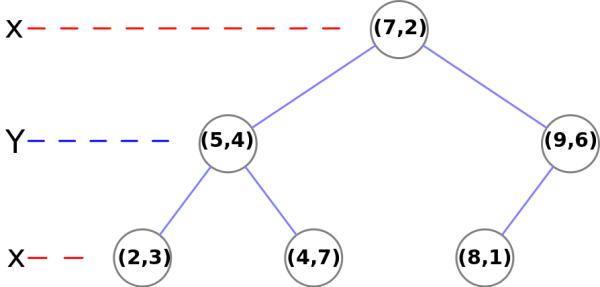
\includegraphics[width=120mm]{../gfx/Tree_0001.png}

% \caption{corresponding-binary-tree}
% \label{fig:tree_0001}
% \end{figure}

% Given that the resulting binary tree is balanced, we get an average search time for the closest neighbor in O(log2(n)) time. For values of k << n, the same average search time can be achieved, with minimal changes to the algorithm, when searching for the k closest neighbors. It is known from literature that balancing the tree can be achieved by always splitting on the meridian node. Building a k-d tree in this manner takes O(kn log2(n)) time.

% Interested readers is encouraged to look at the paper Multidimensional binary search trees used for associative searching by Jon Louis Bentley, where k-d trees first was described.

% \subsection{The serial base algorithm} % (fold)
% \label{ssub:the_serial_base_algorithm}

% \begin{enumerate}
%     \item Build a balanced k-d tree from the point cloud.
%     \item Query the tree for different sets of neighbors.
% \end{enumerate}

% Time complexity:

% Steps:
% \begin{enumerate}
%     \item O(n log2 n). Achieving this speed is dependent on an efficient algorithm for finding the meridian.
%     \item Approximately O(log2 n), but dependent on size of k.
% \end{enumerate}

% \begin{figure}[ht!]
% \centering
% 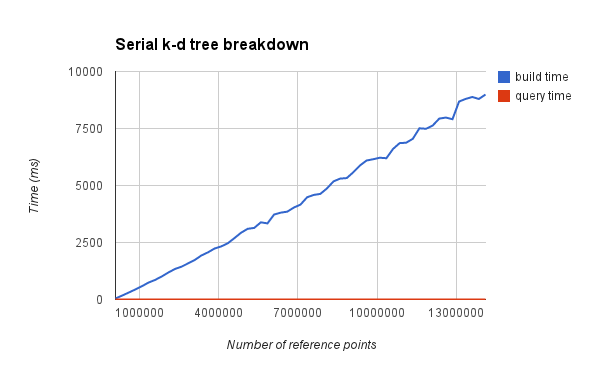
\includegraphics[width=120mm]{../gfx/serial-k-d-tree-breakdown.png}

% \caption{serial-k-d-tree-breakdown}
% \label{fig:serial_kd_tree_breakdown}
% \end{figure}

% Results:

% As expected, almost all the time is spent building the tree. Querying for the closest neighbor in the largest tree took less than 0.0015 ms, but 9 seconds is a long time to wait for the tree to build.

% The paper Real-Time KD-Tree Construction on Graphics Hardware - Kun Zhou et al. offers interesting, although slightly complex, ideas to an efficient parallelization of k-d tree construction. I order to save time, a good amount of time was spent searching for, and trying out, different open source implementations based on this paper. This search was unsuccessful. All the implementations we managed to find was problematic due to lack of updates, often not updated since 2011, and still running on CUDA 4.1, lack of documentation, lack of generalization or dubious source code.

% A more uplifting find was several references to Real-Time KD-Tree Construction on Graphics Hardware in material published by Nvidia, regarding their proprietary systems for ray tracing. A graphics rendering technique often reliant on k-d trees, and indeed dependent on high performance.
% % subsection the_serial_base_algorithm (end)

% \subsection{Our reimplementation} % (fold)
% \label{ssub:our_reimplementation}

% Finding a way to represent the kd-tree boils down to representing a binary tree. This can be done in several ways, but we had some criteria for our representation:

% \begin{itemize}
%     \item The kd-tree should be memory-efficient, at best explicitly storing only the actual point coordinates. This since we want to store the largest possible amount of points on the smaller memory of the GPU.
%     \item The kd-tree representation should be easy to split, distribute and join, since we want to build it on several independent processes.
% \end{itemize}

% After a bit of research and trial and error, we choose to represent the kd-tree as a array of structs, representing points, with an x, y and z coordinate stored in an short array. In order to turn this array into a binary tree, the following scheme was derived. Given an array, the root node of that array is the midmost element (the leftmost of the two, given an even number of elements). To find the left child of the root, you simply find the midmost element of the left sub-array, and likewise for the right child. This representation have some advantages and drawbacks.

% Advantages:
% \begin{itemize}
%     \item Can represent binary trees where not all leaf-nodes are present. This is the minimal requirement for representing perfectly balanced k-d trees.
%     \item Joining or splitting subtrees is as simple as appending or splitting arrays.
%     \item Minimal memory overhead, k-d trees can even be built in-place on the array.
% \end{itemize}

% Drawbacks:
% \begin{itemize}
%     \item Cannot represent imperfectly balanced k-d trees. This mens that the median cannot be calculated through heuristic methods, but enforces a tree optimized for fast queries.
%     \item Location of children and parents have to be recalculated for all basic traversing of the tree, with may reduce the performance of queries on the tree. In order to eliminate this drawback, a index cache is computed before the search is performed.
% \end{itemize}

% Given this representation of the kd-tree, the base kd-tree building algorithm can be expanded to the following:

% Steps:
% \begin{enumerate}
%     \item Find the exact median (of the current split dimension) in this sub-array, and swap it to the midmost place.
%     \item Go through all elements in the list, and swap elements, such that all elements lower than the median is placed to the left, and all elements higher than the median is placed to the right.
%     \item Repeat for the new sub-arrays, until the entire tree is built.
% \end{enumerate}

% Results:

% The serial kd-tree build times was similar or better than the base algorithm, so it is not discussed here

% \begin{figure}[ht!]
% \centering
% 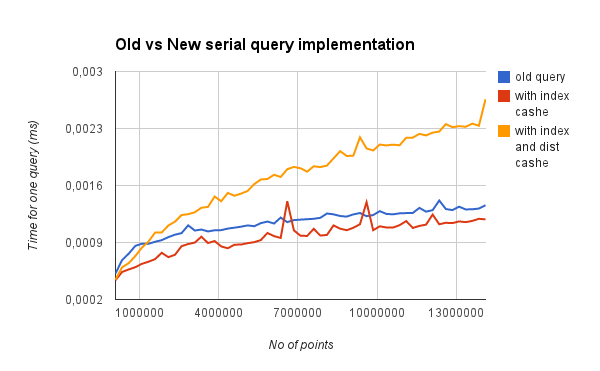
\includegraphics[width=120mm]{../gfx/awg-query-time-old-vs-new.png}

% \caption{Awg query time old vs new}
% \label{fig:awg_query_time_old_vs_new}
% \end{figure}

% The graph shows that our serial implementation of search in this data structure, given a pre-calculated index cache, is as fast, or slightly faster than the base algorithm. The possibility of improving the search even more, by storing all calculated distances in a distance cache was also explored, but we can see from the graph that the overhead associated with this operation did outweigh the benefits.

% Some instability is apparent in the graph, but this is probably due to the author running other programs in the background when performing the test.

% \begin{figure}[ht!]
% \centering
% 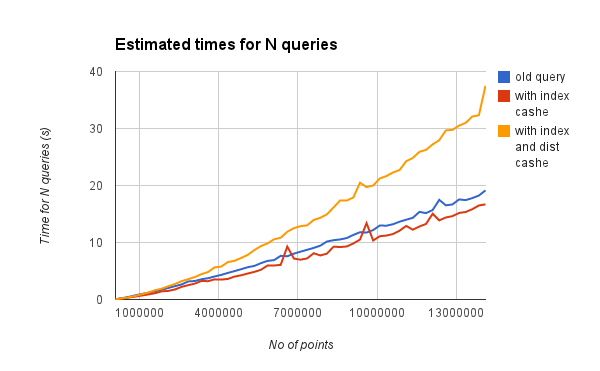
\includegraphics[width=120mm]{../gfx/n-query-time-old-vs-new.png}

% \caption{n query time old vs new}
% \label{fig:n_query_time_old_vs_new}
% \end{figure}

% The trend is exaggerated when considering N searches. Searching with an index cache is overall fastest, and gives a total search time of ~17 s for 14 million searches in a point cloud of 14 million.


% Possible improvements:
% \begin{itemize}
%     \item Run several queries in parallel. Easy to implement, as parallelization is trivial due to independent queries, but is dependent on efficient transfer and storage of the kd-tree on the GPU.
%     \item Explore performance on a variable number of k.
% \end{itemize}
% % subsection our_reimplementation (end)



% % subsection parallel_improvements (end)

% \subsection{V1.4 Release notes} % (fold)
% \label{ssub:v14_release_notes}

% Version 1.4 introduces the possibility of a variable k when searching. Testing the impact of varying the size of k was performed with a fixed number of 1000 repeated single queries. The timing results are shown in the following graph.

% \begin{figure}[ht!]
% \centering
% 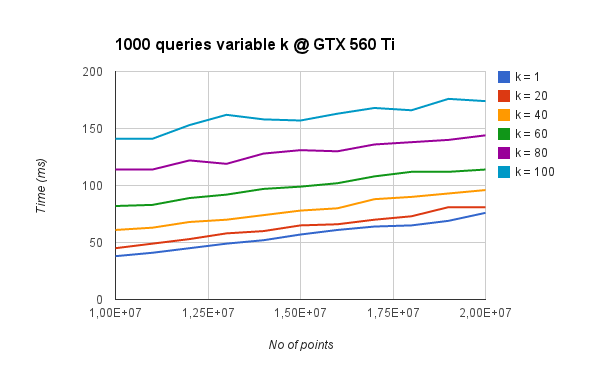
\includegraphics[width=120mm]{../gfx/v14_variable_k.png}

% \caption{Variable k timing results.}
% \label{fig:v14_variable_k}
% \end{figure}

% As expected, increasing k seems to increases the runtime with a constant factor. How this will affect searches in bigger trees and with a larger number of query-points should be explored next.

% Timing tests of the build time and query time for n queries and k = 1 was performed on a GeForce GTX 560 and at Amazon Web Services (AWS). For the GTX card we get the following graph.

% \begin{figure}[ht!]
% \centering
% 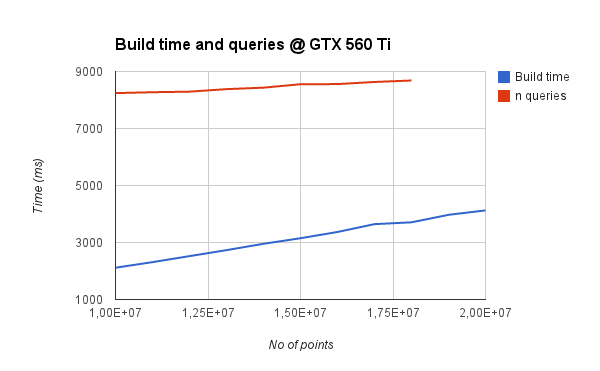
\includegraphics[width=120mm]{../gfx/v14_build_query_gtx.png}

% \caption{Build and query times for v1.4.}
% \label{fig:v14_build_query_gtx}
% \end{figure}

% Querying for n points still takes a lot of time, but the time increase related to the number of points seems to be lower than the build time. This trend is more prominent when we look at the results from our tests on AWS, graphed below.

% \begin{figure}[ht!]
% \centering
% 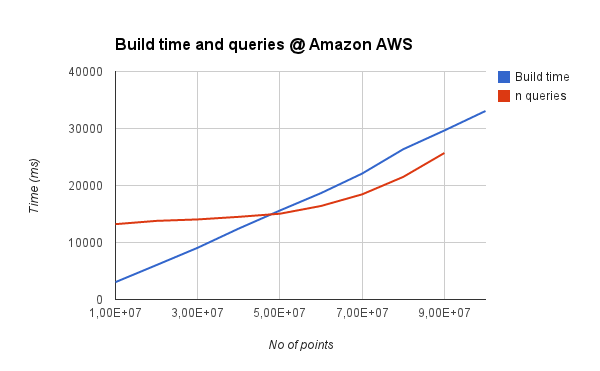
\includegraphics[width=120mm]{../gfx/v14_build_query_aws.png}

% \caption{Build times and queries on AWS.}
% \label{fig:v14_build_query_aws}
% \end{figure}

% Here we see that the runtime for the tree building algorithm catches up with the search time, and surpasses it around 50 million points. This is an interesting result.

% From this graph we can see that on the AWS GPU, we are able, for 90 million points, to build the tree and query for the closest point, k = 1, in a total of ~30s + ~26s = ~56s < one minute.

% Source data for all graphs can be found in
% %[this spreadsheet](https://docs.google.com/spreadsheets/d/1I-qxnPa2FuYs7ePQC7d9v0GVHoYlr4CY6QdJbbNUlYo/edit?usp=sharing).

% % subsection v14_release_notes (end)

% \subsection{V1.3 Release notes} % (fold)
% \label{ssub:v13_release_notes}

% Version 1.3 introduces a couple of new features. Firstly the tree-building algorithm has been updated to also cache the location of the different children of each node in the tree. A small bug related to partition of the point-cloud list was also ironed out. This gives a tree building algorithm whit the following runtime results, comparable with the previous versions of this implementation:

% \begin{figure}[ht!]
% \centering
% 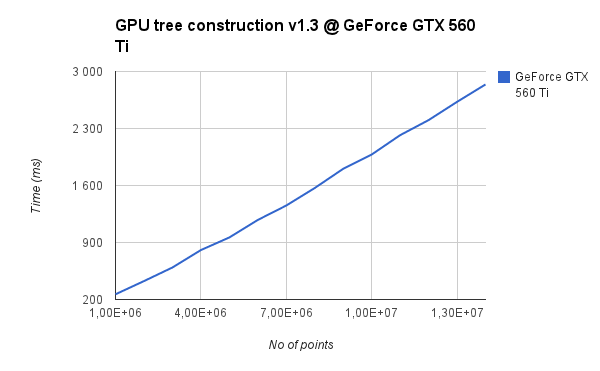
\includegraphics[width=120mm]{../gfx/construction_v13_gtx_560.png}

% \caption{Construction timing results v13 @ gtx 560.}
% \label{fig:construction_v13_gtx_560}
% \end{figure}

% After a surprising amount of fiddling, querying for a large number of query-points was finally parallelized in version 1.3. This gave improved performance when querying many times in the same point cloud. 14 million queries in a point cloud of 14 million points can now be done on average in ~8 seconds. Compared to the estimated ~17 seconds needed by the serial implementation.

% \begin{figure}[ht!]
% \centering
% 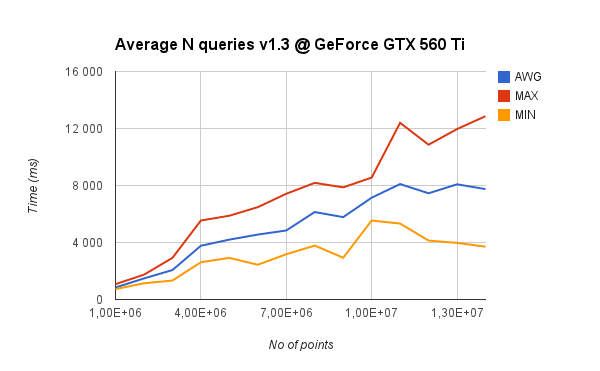
\includegraphics[width=120mm]{../gfx/n_queries_v13_gtx_560.png}

% \caption{n queries timing results v13 @ gtx 560.}
% \label{fig:n_queries_v13_gtx_560}
% \end{figure}

% Unfortunately, this early parallelization gave us quite unstable results. The data in the graph is based on ten timing runs, where the average, minimum and maximum values are collected in three series. As we can see, there is quite a big spread between the best and worst results. Looking at the raw data points for the ten series confirms that this is not a problem caused by a small number of outliers:

% \begin{figure}[ht!]
% \centering
% 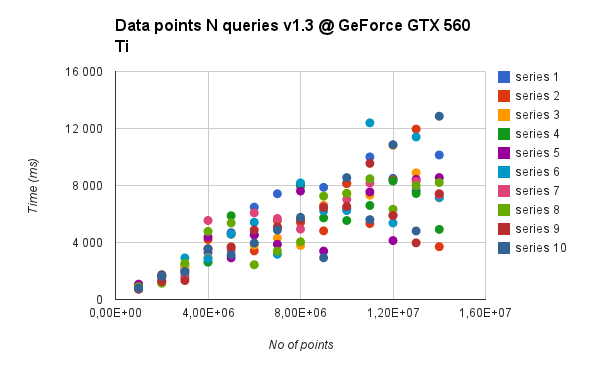
\includegraphics[width=120mm]{../gfx/scatter_n_queries_v13_gtx_560.png}

% \caption{Scatter n queries timing results v13 2 gtx 560.}
% \label{fig:scatter_n_queries_v13_gtx_560}
% \end{figure}

% Some instability would be expected, as the amount of pruning that can be achieved when searching for points in the kd-tree is dependent on the value you search for, but this amount of spread was unexpected. This behavior should be investigated further, as it seems to be indicating some kind of implementation error.

% Combining the results from the search and the tree-building, gives the following runtime for a sequence of building and N queries:

% \begin{figure}[ht!]
% \centering
% 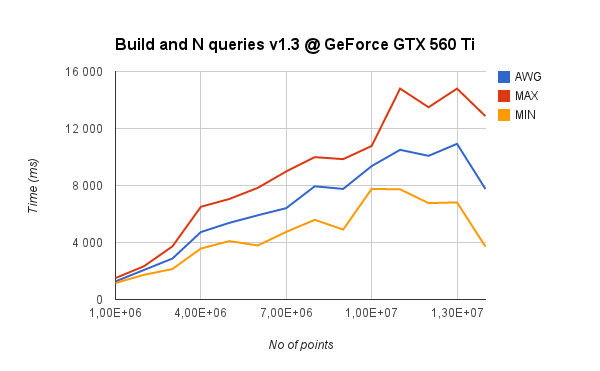
\includegraphics[width=120mm]{../gfx/constructionand_n_queries_v13_gtx_560.png}

% \caption{Construction and n queries v13 @ gtx 560.}
% \label{fig:constructionand_n_queries_v13_gtx_560}
% \end{figure}
% % subsection v13_release_notes (end)
% % section kd_tree_based_effort (end)

\section{Development of a parallel k-d tree algorithm} % (fold)
\label{sec:development_of_a_parallel_k_d_tree_algorithm}


As noted in the previous section, the k-d tree build process is by far the most expensive operation, and we would save a lot of time by managing to parallelize it. One could think, why not use the serial build algorithm. This is a intuitive choice, but in a CUDA context a recursive algorithm is hard to parallelize. CUDA is based on a massive number of lightweight threads, and to get a fast algorithm one have to split the work between as many threads as possible. This is only possible if it is easy to split and divide the work to independent subtasks. In a recursive context this is hard, because a algorithms execution flow in hidden inside a threads call stack. This makes it hard for other threads to get the information needed to participate. The opposite of a recessive algorithm in an iterative approach, with have a more globally accessible execution flow. This introduces a new resource question.

\begin{myrq}
\label{rq:parallel_build}
    It is possible to parallelize the k-d tree build algorithm, in such a way that it gives a significant speed improvement compared to the serial algorithm.
\end{myrq}

In order to investigate RQ \ref{rq:parallel_build}, we have to look a bit closer at the different steps of the k-d tree build algorithm and look at different parallelization strategies.

Steps:
\begin{enumerate}
    \item Find the median of the points along a specified axis. This median point becomes the value of the current node.
    \item Sort all points with lower values than the median to the left of the median, and all the points with higher values than the median to the right.
    \item Perform this algorithm recursively on the left and right set of nodes.
\end{enumerate}

If we analyze the algorithm \ref{alg:seriel_tree_build}, we can see that for each node in the k-d tree a median finding and a partition has to be made, as described in step 1 and 2. We can call this recursive step a node task. The node task has to be done for all nodes starting at the root and successively go down the tree.



\subsubsection{Parallelization strategy} % (fold)
\label{ssub:parallelization_strategy}


First a good overall parallelization strategy has to be found. A good strategy manage to easily split the main task into small individual subtasks. From the serial recursive algorithm \ref{alg:seriel_tree_build}, we see that there are two recursive calls. This is logical, because we are building a binary tree.  The interesting observation is that a node task is only dependent on the parent node tasks. This means that each tree level are independent, which acts as a good start for our parallelization strategy.

Some other small observation, in regard of a parallelization strategy, is that all subtrees in the k-d tree generation are independent. Hence, the tree corresponding to the left and right child of a node can be done in parallel without any communication. The data is also independent, as a result of how we represent the tree as an array. By data independent, it is meant that the data structure easily can be partitioned to each subtask. In our case will the tree array successively be partitioned into contentious sublists, one for each node task.

From these observations, several strategies can be used to parallelize the k-d tree build algorithm. From the first observation a trivial strategy is to divide the tree levels into dependent tasks, where each node task in a tree level is a independent subtask. This gives us an power of two increasing number of parallel nodes tasks as we increase the tree level. The sublist size will decrease with a factor of two in each downward step. An other strategy is to parallelize each node task.

Both strategies can be used in conjunction with each other. The parallel node task algorithm can be used to speed up the early iterations, where the amount of node task in a tree level is small. As well as further parallelize the subtasks in later tree level iterations. This strategy also fit well to our choice of tree representation. One parallel operation can now take the tree array, split the tree into the current subtrees, perform the node task in each subtree in parallel, and the next tree level is created. All can be done inplace, so the algorithm is as memory efficient as possible.


% subsubsection parallelization_strategy (end)

\subsubsection{From recursive to iterative implementation} % (fold)
\label{ssub:from_recursive_to_iterative_implementation}

\begin{algorithm}
\caption{Iterative k-d tree build}
\label{alg:iterativ_tree_build}
\begin{algorithmic}
    \Function{Build-KD-Tree}{$Tree$}
        \ForAll {$level \in \text{all levels in } Tree$}
            \ForAll{$node \in level$}
                \State $dimension \gets |level| \bmod k$ \Comment{k = 3 for a three dimensional k-d tree}
                \State $\text{Balance-node}(node, dimension)$
            \EndFor
        \EndFor
    \EndFunction
\end{algorithmic}
\end{algorithm}


% subsubsection from_recursive_to_iterative_implementation (end)




% TODO: Header must be improved
\subsubsection{Selecting an algorithm} % (fold)
\label{ssub:selecting_a_algorithm}



As we have seen in section \ref{sub:application_of_kd_trees_to_the_knn_problem}, many algorithms for finding median exist. Since we now want to implement the algorithm with CUDA, the environment has changed, and quick select may not be the best alternative anymore. The first problem with quick select is that it is recursive, which makes it hard to parallelize on CUDA. Therefor it may be profitable to look at other, more parallelization, algorithms.


First a reuse of the bitonic sort was investigated. Given a sorted list one can find the median directly, by simply looking at the midmost element of the array. The partitioning is also done in the process. Unfortunately this strategy proved unsuccessful, as re-purposing the bitonic algorithm for such an task proved difficult. The reason for this is that a pure bitonic sort only manage to sort lists with a length of power of two. The normal solution is to create a longer list then needed, which destroys many of the advantages with our binary tree representation. There are also other solutions to the problem, for example one by K.E. Batcher \cite{Batcher:1968}, but these solutions introduces a lot of divergence that destroys performance on the GPU. We also have the inherent downside of sorting a list in order to find the median, since \BigO{n} algorithms for finding the median exist, compared to the \BigO{n log(n)} time required by sorting.


The existing linear algorithms for finding the median is mostly based on a more generic problem, namely selection or k'th order statistic algorithms \citep[Chapter 9]{Cormen:2001}. Our serial choice, Quick select, is one of these. It is possible to implement a iterative version, so that the bad properties from the recursive version are eliminated. This option was ignored, because literature states that there are other better suited algorithms, like Alabi \citep{Alabi:2012}. Alabi goes through the radix select and bucket select algorithm in detail. The big difference between them is the constant time penalty. The radix sort have a more exact time complexity of \BigO{bn}, where b is the number of bits in each number. While the penalty for bucket select is \BigO{an}, where $a$ stands for the degree of agglomeration in the values. The algorithm is week when the points are clusters together. His results shows that bucket select normally is slightly faster, except when $a$ is high. Although bucket select normally have better results, we expect a high degree of agglomeration in our application, so we choose radix select.


\subsubsection{Radix select} % (fold)
\label{ssub:radix_select}

% subsubsection radix_select (end)

The radix select is based on a bitwise partitioning, much like radix sort \cite[Chapter 8.3]{Cormen:2001}. In each step, elements are partitioned in two subgroups based on the current bit. Then the subgroup that contains the median is determined, and the search continue in that subgroup until the median is found.

\begin{figure}[ht!]
\centering
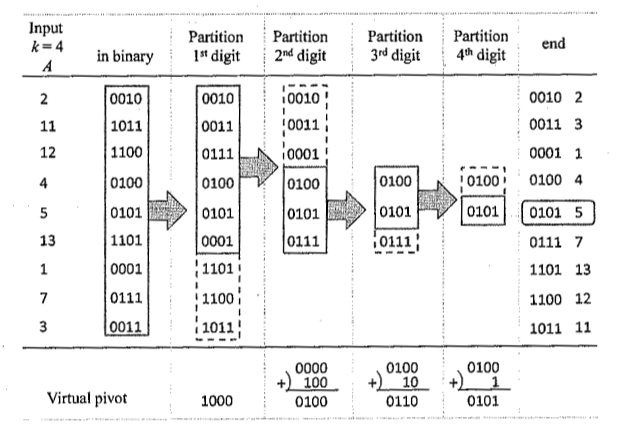
\includegraphics[width=100mm]{../gfx/Radix_select.png}

\caption{An illustration of radix selection \cite{cayman:2012}.}
\label{fig:radix_select}
\end{figure}

When it comes to create a parallelization strategy for radix select it is first advisable to take a look at a highly optimized radix sort like, \citep{MerrillG11}. The radix select can easily be reduced from a radix sort, and many concepts can therefore be reused. An other interesting implementation is the radix select from \citep{Alabi:2012}. They both uses a intuitive parallelization strategy by splitting each radix partition into parallel operations. The way our and Alba's solution differs from Merrill is firstly that we start on the most significant digit, since a least significant digit approach will not reduce the problem in each step. Secondly we only iterate on the digit which contains the median, and let us reduce the problem in each iteration.

Our radix select is a slightly modified version in three ways. We want to solve the node task, which forces us to also partition the list around the median. The algorithm also need to work in a inplace fashion. The last modification, is that our parallel operation must to several radix selections at once, at different parts of the main tree array.


\subsubsection{Our implementation} % (fold)
\label{ssub:our_implementation}


- split up the work in respect to cuda
- Pseudocode
- forklarting av cuda
- diskutere minnebruk. shared memory
- divergence
-



% subsubsection our_implementation (end)





% It is hard to use all the parallel power of cuda in this algorithm. The reason is that the problem is divided in three different types; partition one huge list, partition some middle sized list and partition many small lists. This is the reason why we have chosen to use three different implementation of k'th order statistic. The constant time penalties of the two algorithms we have chosen give us a clear indication the radix select is best on large lists while quick select is best on small lists.

% Results:
% \begin{figure}[ht!]
% \centering
% 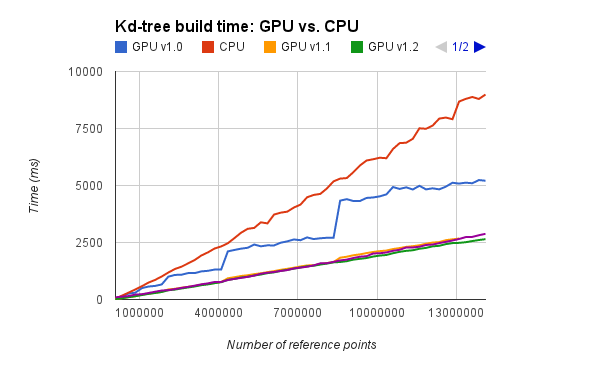
\includegraphics[width=120mm]{../gfx/gpu-vs-cpu-build-time.png}

% \caption{GPU vs CPU build time.}
% \label{fig:sublime_ide}
% \end{figure}

% We see that the parallel implementation performs better than the base serial implementation, building a tree of 14 million points in just over 5 seconds, compared to just under 10 required by the serial algorithm. Still we regard this as a quite rough implementation, in need of more tuning to really bring out the speed potential. The potential for parallelizing the workload for the first and last iterations have not been fully developed. This is due to the implementation forcing one version of the radix select algorithm being to work on all problem sizes. This is not optimal for dividing cuda resources, and as a result, we get high penalties when the problem size reaches unsuitable values.

% We also see a couple of large jumps in the graph. This happens when the number of elements passes a power of two and the height of the resulting k-d tree increase. The height increase hits the implementation at its weakest.

% Tuning the algorithm to alternate between radix select and quick select, eliminates this problem, as is visible in the graph for GPU v1.1. This removes the penalty for calculating the median at unsuitable problem sizes, giving an build time of ~2.4 seconds for 14 million points, compared to the ~9 seconds required by the serial implementation, or the ~5.2 seconds required by the old parallel implementation.

% % subsubsection selecting_a_algorithm (end)
% Memory usage:

% To analyses the space complexity of the k-d tree build and search algorithm, we have made an theoretical calculation of both algorithms GPU memory consumption, and tested it against results from a GeForce 560ti and a Nvidia grid K520 (amazon web service delved).

% It is important to note that the only hard memory limitation is related to building the tree, as a search for N query-points can be performed in several operations. If you e.g. run into memory limitations when searching for pow(10, 8) query-points, you can simply perform two searches on pow(5, 8) query-points to get around the limitation. Loading the pre-built k-d tree on the GPU for searching, and performing one query for a low value of k, will always consume less memory than building the actual k-d tree.

% **Kd-tree-build**

% The memory consumption for the k-d tree build is only depended on the number of points (n) and the theoretical consumption rate grows linearly as \BigO{36n} subset of \BigO{n}.

% \begin{figure}[ht!]
% \centering
% 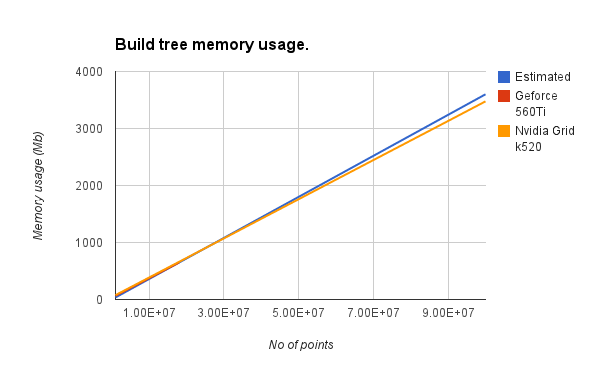
\includegraphics[width=120mm]{../gfx/memory-usage-build.png}

% \caption{Memory usage of k-d tree-build.}
% \label{fig:memory_usage_build}
% \end{figure}

% We see that the estimation fit the real consumption almost perfectly, and with this memory model, we can easily estimate the GPU memory requirements for different problem sizes.

% Given that a customer wants to perform a knn-search on a point cloud of 100 million, he or she would need a GPU with at least 3.6 Gb of spare memory. Under we have tabulated what maximum problem sizes you would expect to be able to run on a selection of Nvidia graphics cards:

% \begin{center}
%     \begin{tabular}{ | l | l | p{5cm} |}
%     \hline
%     Nvidia GPU & Available memory & Maximum problem size \\ \hline
%     GTX TITAN & 6144 MB & 1.79E+08 \\ \hline
%     GTX 780 & 3072 MB & 8.95E+07 \\ \hline
%     GTX 770 & 2048 MB & 5.97E+07 \\ \hline
%     Quadro K6000 & 12288 MB & 3.58E+08 \\ \hline
%     Quadro K5000 & 4096 MB & 1.19E+08 \\ \hline
%     Quadro K4000 & 3072 MB & 8.95E+07 \\ \hline
%     Tesla K40 & 12288 MB & 3.58E+08 \\ \hline
%     Tesla K20 & 5120 MB & 1.49E+08 \\ \hline
%     \end{tabular}
% \end{center}

% These numbers should be read as rough estimates, as each card is expected to have internal processes requiring an unspecified constant amount of the available memory, therefor lovering the maximum problem size possible to run on these cards in practice. It is also worth to mention that when buying a GPU for GPGPU tasks, other performance characteristics is equally, or more, important.

% **Kd-search**

% The kd-search is used to query every point against each other. It has a theoretical memory consumption rate at \BigO({40+4k}n) subset of \BigO{kn}. The consumption is therefore depended on the number of points (n) and the number of neighbors (k).

% \begin{figure}[ht!]
% \centering
% 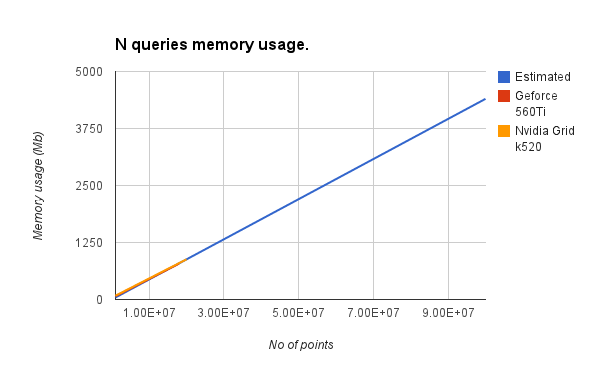
\includegraphics[width=120mm]{../gfx/memory-usage-kd-search.png}

% \caption{Memory usage of kd-search.}
% \label{fig:memory-usage-kd-search}
% \end{figure}

% Also in this case our estimation fit the real consumption with a high degree of accuracy.

% Further work:
% \begin{itemize}
%     \item Look at memory optimization.
%     \item Improve utiliti methods like: accumulateindex, minReduce.
%     \item Forloop Unrolling.
% \end{itemize}

% section development_of_a_parallel_k_d_tree_algorithm (end)

\section{Development of a parallel k-d search algorithm} % (fold)
\label{sec:development_of_a_parallel_k_d_search_algorithm}






% Antar begreper qknn har blitt intodusert

Now that a parallel k-d tree build algorithm has been build, lets start looking into a parallelization of the qkNN operation. Some question immediately arise. What is the best way to parallelize such a problem? Will a GPU version give a beneficial speedup? This leads to a new resource question that acts as an expatiation of RQ~\ref{rq:serial-kd-tree}.


\begin{myrq}
\label{rq:parallel_query}
    It is possible to parallelize the qkNN query algorithm, in such a way that it gives a significant speed improvement compared to the serial algorithm.
\end{myrq}


To investigate RQ~\ref{rq:parallel_query}, a real world test and implementation is always beneficial, but first some resource and discussion is needed. Especially in what kind of parallelization strategy and algorithm that should be used. Maybe the GPU is not the right way to parallelize this kind of operations.


\subsection{Parallelization strategy} % (fold)
\label{sub:parallelization_strategy}


The problem at hand is the qkNN search, which is where an assumed big number of query's is to be performed on a k-d tree. At first glance this looks good in terms of parallelization. The main task is naturally divided into individual subtasks, namely the queries. This is a perfect parallelization example, where any number of threads independently can move up and down a constant tree structure.

When CUDA and implementation related questions is introduced, some interesting aspects needs to be addressed. The first is how the work should be divided in terms of CUDA resourced. Should one query be done in a block, should each thread to one query or maybe we should use one thread per $k$ in a query. To address this question, one need to be able to determent if a query itself can be parallelized.

First we see that a query does not have many node visits compared to the size and presumably the number of queries. This ratio is based on the binary logarithm, as for example a tree with one million elements and a $k$ equals one, the number of visited nodes is proportional to $20$. This indicated that many threads is not as beneficial. The relative hard problem of parallelize a query is also a good indicator. Parallelization is, as we have discussed earlier, dependent on individual subtask. The query task is heavily dependent, as the next node is determinant on the previous node. The only place independence comes into existents is where left and right subtree is to be searched, but if this is parallelized the benefit of the pruning is partially destroyed. This leads to one conclusion, if threads is not to be wastefully used, one thread per query is required. In terms of independent tasks, the one thread approach is also logical, since the number of queries should outperform the number of cores on the GPU\@.

The overall parallelization strategy is therefore to use one thread per query and equally distribute the queries amongst the GPU's SM\@.


\subsection{Problem with the recursive implementation} % (fold)
\label{sub:problem_with_the_recursive_implementation}

As discussed in previous sections, GPU's and recursion don't get along well. Previously some drawbacks were mentioned, including the disability for thread communication. Since our parallelization strategy new states that all threads do individually work and don't need to communicate, is there steal a reason for a iterative conversion.

One aspect to consider is connected to how the GPU hardware is constructed. The GPU have a lot of lightweight threads, and has therefor not as mush local space or caching as in a CPU\@. This means that the call stack, where the instructions are manged, is relatively small. A recursive algorithm adds instructions on this call stack at each recursive call. This is the reason why the executions flow of a recursive algorithm is hidden, the call stack is not reachable from the programmers point of view. The big question here is wherever the call stack on a CUDA GPU is big enough for our application.

This question was investigated by a trail and error method, since its hard to do the explicit calculations. The call stack is located locally, so results from a block should be enough. To test the limitations a test that spawned $64$ theoretical threads on an increasing tree size should be sufficient. As the tree size passed \numprint{1e5}, we stared to get unknown errors from CUDA\@. This we concluded was the leak of call stack space and concluded that CUDA had a to small call stack for our purpose.


Divergence is also an accept to consider, and in this case execution divergence. This is, as mention before, then the execution of threads in a warp differs. In a recursive algorithm the decision of whether a recursive call should be made or not, is entirely up to a single thread. Once two threads have made different desiccation, there is no guaranty that they will stay in sync.

The execution divergence can be solved by en iterative solution, where one is guaranteed that every thread always stay in sync. An iterative approach will also solve the call stack problem, where the recursion stack is explicitly stored. The transformation is therefor a necessity.


% subsection problem_with_the_recursive_implementation (end)

\subsection{From recursive to iterative implementation} % (fold)
\label{sub:from_recursive_to_iterative_implementation}


To rewrite Algorithm~\ref{alg:recursive_knn_kd_tree_search} into a iterative algorithm by  explicitly managing the recursion stack, some properties about how the search traverse the k-d tree is needed. From Algorithm~\ref{alg:recursive_knn_kd_tree_search} one can see that this is an inorder traversal, since the current node work is node between the recursive calls. This traversal in also the best strategy in a binary tree search, because the pruning of subtrees is maximized. How to make a standard binary search tree in an iterative fashion is described in Cormen\cite[Chapter 12]{Cormen:2001}, but since this is a k-d tree search the implementation is slightly different, as shown in Algorithm~\ref{alg:iterative_knn_kd_tree_search},

\begin{algorithm}
\caption{Iterative kNN k-d tree search}
\label{alg:iterative_knn_kd_tree_search}
\begin{algorithmic}
    \Procedure{Iterative-kNN-KD-Tree}{$K, r, q$}
        \State \text{Let $S$ be a stack for collecting tree nodes}

        \State $i \gets 2$

        \While{$!S.empty$ \textbf{or} $r$ != NIL}
            \If{$r$ = NIL}
                \State $r \gets \Call{Pop}{S}$
                \State $i \gets r.dimension$

                \If{$r.dx^2 < K.max$} \Comment{Can there be closer points in the other subtree?}
                    \State $r \gets r.other$
                \Else
                    \State $r \gets \text{NIL}$
                \EndIf
            \Else
                \State $d \gets \Call{Distance}{r, q}$

                \If{$d < K.max$} \Comment{Is $r$ closer to $q$ than the current k best points?}
                    \State $r.distance \gets d$
                    \State $\Call{Insert}{K, r}$
                \EndIf

                \State $i \gets (i + 1) \bmod k$ \Comment{k = 3 for a three dimensional k-d tree}

                \State $r.dimention \gets i$
                \State $r.dx \gets r.x(i) - q.x(i)$

                \If{$r.dx > 0$}  \Comment{Select $t$ and $o$ so we traverse towards closest point first}
                    \State $t \gets r.left$, $r.other \gets r.right$
                \Else
                    \State $t \gets r.right$, $r.other \gets r.left$
                \EndIf

                \State $\Call{Push}{S, r}$
                \State $r \gets t$
            \EndIf

        \EndWhile
    \EndProcedure
\end{algorithmic}
\end{algorithm}

The algorithm works in the same way as the recursive algorithm, but adds a stack, $S$, called the s-stack, and a while loop in order to handle the tree traversal iteratively. While there is a element assigned to the root variable, $r$, the algorithm will traverse down the target branch, updating the dimension, $i$, calculating the distance, $dx$, determining the target, $t$, and other, $o$, child node. Then it will collect $r$, $o$, $i$ and $dx$ into one element, and push it on the s-stack. Finally the root variable is assigned to the target child, or NIL if we have reached the end of a branch.

While there still is elements in the s-stack, but $r$ is assigned to NIL, we are traversing back up a branch. While this is happening, the algorithm pops elements from the s-stack, determines if they should be added to the k-heap, before it determines if it need to investigate the other branch of this node. If that is the case, the other node is assigned to $r$, and the algorithm will traverse down this subtree using the previously stated rules.


% subsection from_recursive_to_iterative_implementation (end)

%TODO: Forandre header?
\subsection{The implementation} % (fold)
\label{sub:the_implementation}

To convert our iterative search algorithm to CUDA should now be a trivial matter. The code itself does not need to be parallelized, as only one thread is used per query. The final implementation can be found in Appendix~\ref{sec:cuda_k_d_tree_search} Some key aspects is wort highlighting.


As we converted the algorithm from a recursive to a iterative stack based solution, a lot of the problematic divergence was taken avoided. But as shown in Algorithm~\ref{alg:iterative_knn_kd_tree_search}, there is steal some divergence. This is inevitable since the target subtree and other subtree needs to be treated differently. Although, there are possibilities to minimize the thread branching. If threads in a warp is traversing completely different parts of the tree, they will access different nodes. This is called data divergence. They will also be a minimal change for the threads to synchronize there target and other traversing. The solution is to let each warp search for points that are close in 3-d space, which will force the threads to traverse fore or less together. In our application, query for all points in the k-d tree, this is an easy task. When the k-d tree was build the points are, due to the data structure and the nature of a k-d tree, grouped together relatively to their position in space. The divergence will therefore be minimized if the points are fed to the search as they are placed in the k-d tree.


The transformation from a hidden recursive stack to a explicit stack makes a interesting question about where to store the new stack, especially
since it definitely would have overfilled the local call stack space. This is data that are modifiable and thread independent, which means that the memory options are shared memory, local memory and global memory. Local memory is the memory each thread dynamically can allocate from the heap. First of all, global memory is a working candidate. It has enough space, it is modifiable and accessible to all threads. The huge drawback is the access time, it takes around $400$ clock cycles(Trenger vi cite), and it would be beneficial to use some other kind of memory. Shared memory would be a perfect candidate, because the memory is fast and the need to communicate between blocks is nonexistent. The only drawback needed to address the the amount of data available in shared memory, which is default around $49 kb$ for each block on current NVIDIA GPU's. This is also a good approximation for how much local memory available.

The two stacks in question is the k-stack and the transformed recursive stack, called stack from now on. Both stacks are memory wise dependent on number of threads, since each thread needs unique stacks. The stack is dependent on how many elements the inorder tree traversal needs to store. If one looks on how the algorithm handles the stack, one can see that elements are pushed on the way down, and poped when one traverse upwards.  This means that the stack never will be longer then the tree hight, which is the binary logarithm if the size. One stack element uses $16$ bytes of space, which means that the stack memory is s subset of $\Theta(16\log_2(n)T)$. Here $T$ represent the number of threads and $n$ is the k-d tree size. The k-stack depends on the number of closest neighbors, $k$, and one element uses $8$ bytes. This implies that it uses memory usage will look like, $\Theta(8kT)$.


\begin{figure}[ht!]
\centering
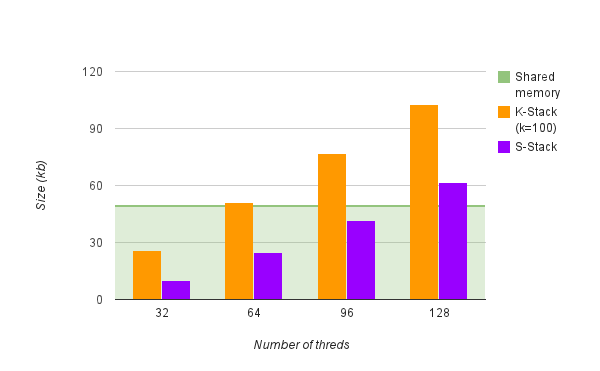
\includegraphics[width=100mm]{../gfx/shared_memory_and_stack.png}

\caption{The stacks memory usage compared to the amount of shared memory.}
\label{fig:stacks_and_shared_memory}
\end{figure}


In Figure~\ref{fig:stacks_and_shared_memory} the memory usage of each stack is compared to the available shared memory. Some basic assumptions and approximations have been done in regard to the data. Treads are only compared in multiples of $32$, since this is the warp size and is therefore the most optimal thread numbers. The value of $k$ is dependent on the problem in hand, and as our application only needs a value of $100$, that value is used. When it comes to the logarithm in the stack calculations, we have chosen $30$.  This is because it value is relatively constant and with a value of this type we support a \numprint{1e9} big k-d tree.


Figure~\ref{fig:stacks_and_shared_memory} shows that the k-stack is not a suitable candidate. Already at a thread count of $64$ the memory is used. The highly dependent and variably $k$ value also make the stack size unpredictable. The stack however looks really promising, with $64$ threads the memory usage is well below the limit. This also shows that local memory a suitable candidate, since it allocate memory from the same L1 chip as the shared memory.

\begin{figure}[ht!]
    \centering
    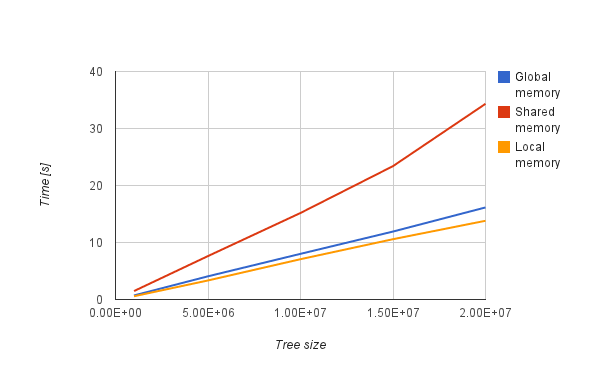
\includegraphics[width=100mm]{../gfx/stack_speed.png}

    \caption{Speed comparison between different stack memory types. The test are done with $k$ equals 10 and \numprint{1e6} queries per tree size. }
    \label{tbl:stack_speed}
\end{figure}



To decide what kind of memory is optimal for our stack, Figure~\ref{tbl:stack_speed} has been created. Surprisingly shared memory looks like the slowest alternative, even though the two other should be stored in global memory. Shared memory is synced between all threads in a block, and may have some of the blame for our results. One property of the stack is that it is completely thread local, meaning communication between threads is not needed. The extra, and wasted property of the shared memory may lead to to a decrease in latency, because data is synced between the threads.

An other reason is that there is some kind of programming error, and some part of a stack was used by two threads. This would lead to a lot of write and read collisions, and cause a lot of time penalties. The programming error would also lead to wrongly results, which is not the case and the error possibility is ignored.

Although global and local memory presumably is stored at the same place, the are some noticeable differences that can explain the time gap between them. The cache may be a noticeable factor. The cache is is placed on the same on-chip memory as the shared memory, and should therefore be equally fast. The difference is that cashing is not programmable and therefor not controlled be the programmer. However some properties in the local memory type may suggest that it is a more likely candidate to be cached.  The local memory is thread dependent and is not accessible to other threads or blocks as the global memory are. The compiler can therefor logically imply that the data is not modified by other threads and caching becomes mush more likely. Figure~\ref{fig:stacks_and_shared_memory}, also shows us that the cache can fit all stacks in a block, which correlates with the timing results. To enforce cache use even further CUDA gives a runtime function call to give more of the on-chip memory to caching.

The discussion and results for the stack analysis shows that the stacks highly impact the timing results. This means that the k-stack is also a dominant  speed factor, as corresponds well to the k-stack tests that was performed. Two k-stack variants was tested. One that used a bobble sort\cite{Cormen:2001} like implementation. It works by always keeping a sorted list. An element is inserted by, from the bottom position, swapping it to the adjustment element until it is in the right place. The other method is based on a heap sort implementation, that is explained in Section~\ref{sub:querying_the_k_d_tree}. The timing difference between the two implementations was around $5$ times. The fastest one was of course the heap-sort variant, since it need to access mush less elements. The difference is the insertion time complexity, where the bobble variant is a \BigO{n} and the heap sort variant is a \BigO{log_2(n)}.


\subsubsection{Open-MP} % (fold)
\label{ssub:open_mp_version}

The high impact the stack had on performance make an interesting question in regard to RQ~\ref{rq:parallel_query}. Could a parallel implementation in the CPU outperform the CPU version? When the latency effect, as the stacks showed, had such a huge impact on the performance. The CPU has a lot more cache then the GPU and would therefor not be affected that mush. The real question is whether the CUDA implementation manges to hide the latency problem by alternating between different warps.

For this to be investigated properly, an OpenMP version of the k-d tree search has to be created. Parallelization wise this is not as different as in our CUDA discussion, and there are only some implementation details to address. The big discussions around what kind of memory to use or memory size can also be ignored, since the CPU has enough cache and the latency is not that important. The implementation can be found in Appendix~\ref{sec:open_mp_k_d_tree_search}.

% subsubsection open_mp_version (end)


% subsection our_implementation (end)











% \begin{figure}[ht!]
% \centering
% 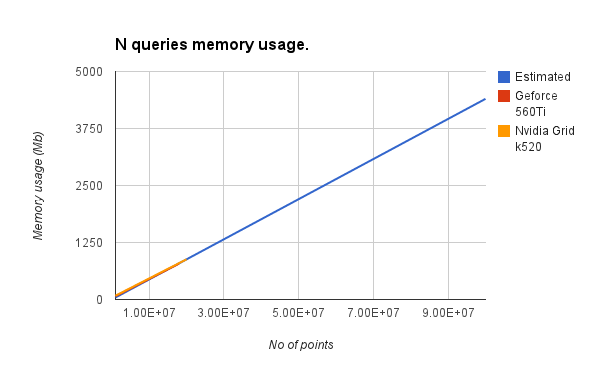
\includegraphics[width=120mm]{../gfx/memory-usage-kd-search.png}

% \caption{Memory usage of kd-search.}
% \label{fig:memory-usage-kd-search}
% \end{figure}

% Also in this case our estimation fit the real consumption with a high degree of accur
% Further work:
% \begin{itemize}
%     \item Look at memory optimization.
%     \item Improve utiliti methods like: accumulateindex, minReduce.
%     \item Forloop Unrolling.
% \end{itemize}





% section development_of_a_parallel_k_d_search_algorithm (end)

\subsection*{Cuda Optimizations}

\begin{enumerate}
\item 32 threads in a warp
\item Number of threads and blocks. Calaculate on each lounch
\item divergence
\item memory placement
\item
\end{enumerate}

\cleardoublepage
